%
\documentclass[a4paper]{article}

\usepackage{xcolor}
\pagecolor{yellow}
\usepackage{tikz}
\usepackage[margin=.0cm, bottom=15pt, left=1.4cm, right=1.4cm, top=-.2cm]{geometry}
\renewcommand{\familydefault}{\sfdefault}
\setlength{\parindent}{0pt}
\usetikzlibrary{calc,shapes.callouts,shapes.arrows}
\usetikzlibrary{shadows.blur}
\begin{document}

\hspace{-1.4cm}

\includegraphics[width=10cm]{full-colour-logo}
\hfill
\raisebox{.5cm}{\begin{minipage}[b]{0.6\textwidth}
\raggedright
{\bf \Huge PhD Opportunities}
\\[-4pt]
\Huge \em in the Theory Group,
\\[-4pt]
School of Computer Science
\end{minipage}}

\vspace{-8pt}
\LARGE\raggedright
We are one of the \textbf{largest research groups in the world} to focus on the logical foundations of computer science.

\[
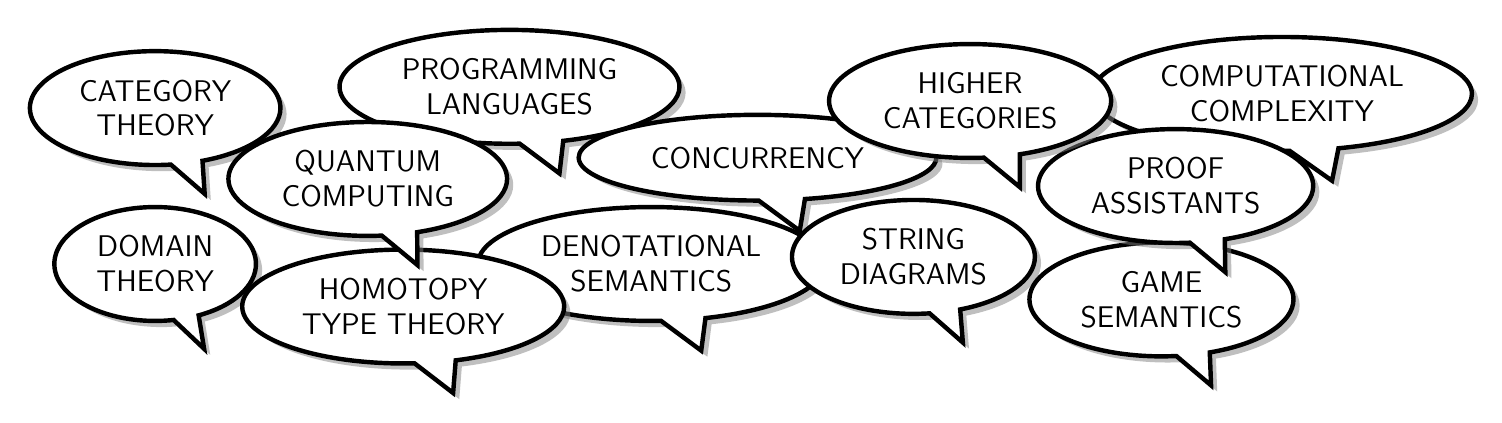
\begin{tikzpicture}[scale=.9]
\tikzset{sp/.style={align=center, ellipse callout, fill=white, draw, ultra thick, drop shadow, font=\large, inner sep=5pt, scale=.9}};
\node [sp] at (0,0) {PROGRAMMING\\LANGUAGES};
\node [sp, inner sep=8pt] at (3.5,-1) {CONCURRENCY};
\node [sp] at (2,-2.5) {DENOTATIONAL\\SEMANTICS};
\node [sp] at (-5,-2.5) {DOMAIN\\THEORY};
\node [sp] at (10.9,-0.1) {COMPUTATIONAL\\COMPLEXITY};
\node [sp] at (5.7,-2.4) {STRING\\DIAGRAMS};
\node [sp] at (-5,-.3) {CATEGORY\\THEORY};
\node [sp] at (-1.5,-3.1) {HOMOTOPY\\TYPE THEORY};
\node [sp] at (9.2,-3) {GAME\\SEMANTICS};
\node [sp] at (-2,-1.3) {QUANTUM\\COMPUTING};
\node [sp] at (9.4,-1.4) {PROOF\\ASSISTANTS};
\node [sp] at (6.5,-.2) {HIGHER\\CATEGORIES};
\end{tikzpicture}
\]


%\vspace{-30pt}{\bf \Huge Staff}

\newcommand\staff[3]{\tikz{
\path [use as bounding box] (-1,-1) rectangle +(8.8,2.2);
\node at (0,0) {\includegraphics[width=2cm]{photos/#2}};
\node [anchor=west, font=\bf] at (1.1,0.6) {\vphantom{|}#1};
\node [anchor=north west, font=\em, align=left, text width=8cm, scale=.8] at (1.1,0.3) {\vphantom{|}#3};
}}

\staff{Benedikt Ahrens}{ahrens.jpg}{Higher categories, homotopy type theory, proof assistants}
\staff{Miriam Backens}{backens}{Quantum computation, complexity theory, string diagrams}
\staff{Rajesh Chitnis}{chitnis}{Algorithms and complexity,\\game theory}
\staff{Anupam Das}{das}{Proof theory, logic, complexity theory}
\staff{Martin Escardo}{escardo}{Homotopy type theory, proof assistants, topology}
\staff{Dan Ghica}{ghica}{Programming languages, string diagrams, game semantics}
\staff{Achim Jung}{jung}{Programming languages, domain theory, philosophy of computing}
\staff{Nicolai Kraus}{kraus}{Higher categories, homotopy type theory, proof assistants}
\staff{Paul Levy}{levy}{Programming languages, game semantics}
\staff{Dave Parker}{parker}{Verification, model checking}
\staff{Vincent Rahli}{rahli}{Programming languages,\\verification, proof assistants}
\staff{Uday Reddy}{reddy}{Programming languages, logic, proof theory}
\staff{Eike Ritter}{ritter}{Verification, model checking}
\staff{Jamie Vicary}{vicary}{Quantum computing, higher\\category theory}

\vspace{10pt}
Full bursaries are available for UK\ and EU\ students.

We also support applications for outside scholarships.

\vspace{5pt}
\textbf{www.cs.bham.ac.uk/research/theory}

\end{document}
